\documentclass[a4paper, 12pt]{article}

\usepackage{a4wide}
\usepackage[utf8]{inputenc}
\usepackage[russian]{babel}
\usepackage[pdftex]{graphicx}
\usepackage{amsmath}
\usepackage{amssymb}
\usepackage{amsfonts}
\usepackage{graphicx}
\usepackage{hyperref}
\usepackage{verbatim}
\usepackage{indentfirst}
\usepackage[left=3cm, right=1.5cm, top=2cm, bottom=2cm]{geometry}
\usepackage{listings}
\setlength{\parindent}{1.25cm}
\linespread{1.3}
\setcounter{page}{2}

\newtheorem{myComment}{Замечание}
\newtheorem{myDef}{Определение}
\newtheorem{myProp}{Свойство}
\newtheorem{myTeor}{Теорема}
\newcommand{\dbtilde}[1]{\accentset{\approx}{#1}}
\DeclareMathOperator{\sign}{sign}

\begin{document}

\thispagestyle{empty}

\begin{center}
\vspace{-3cm}

\includegraphics[width=0.5\textwidth]{src/msu.png}\\
{\scshape Московский государственный университет имени}\\
М. В. Ломоносова\\
Факультет вычислительной математики и кибернетики\\
Кафедра системного анализа

\vfill

{\LARGE Ашабоков Аслан Нажмудинович}

\vspace{1cm}

{\Huge\bfseries Отчёт по теоретическому заданию в рамках курса
«Суперкомпьютерное моделирование и технологии»}\\

\vspace{1cm}

{\LARGE ЗАДАНИЕ 1}
\end{center}

\vspace{1cm}

\begin{flushright}
  \large
  \textit{Студент 615 группы}\\
  А.\,Н.~Ашабоков

  \vspace{5mm}

%  \textit{Научный руководитель}\\
%  к.ф.-м.н., доцент П.А. Точилин
\end{flushright}

\vfill

\begin{center}
Москва, 2021
\end{center}

\newpage
\setcounter{tocdepth}{2}
\tableofcontents

\newpage
\normalsize

\section{Построение информационного графа}

	В рамках данной работы был построен информационный граф следующего фрагмента кода на языке Си:
	
	\lstset{language=C}
	\begin{lstlisting}
	for(i = 2; i <= n+1; ++i)
	  C[i] = C[i - 1] + D[i];
	for(i = 2; i <= n+1; ++i)
	  for(j = 2; j <= m+1; ++j)
	    B[i][j] = B[i][j];
	for(i = 2; i <= n+1; ++i){
	  A[i][1][1] = B[i][m + 1] + C[n + 1];
	  for(j = 2; j <= m+1; ++j)
	    for(k = 1; k <= n; ++k)
	      A[i][j][k] = A[i][j - 1][k - 1] + A[i][j][k];
	\end{lstlisting}
	
	Xml-описание графа имеет вид:
	
	\lstset{language=xml}
	\begin{lstlisting}
<?xml version="1.0" encoding="utf-8"?>
<algo>
    <params>
        <param name = "N" type = "int" value = "4"></param>
        <param name = "M" type = "int" value = "5"></param>
    </params>

    <block id = "0" dims = "1">
        <arg name = "i" val = "2..N+1"></arg>

        <vertex condition = "" type = "1">
            <in src = "i - 1"></in>
            <in bsrc = "-1" src = "i"></in>
        </vertex>
    </block>

    <block id = "1" dims = "2">
        <arg name = "i" val = "2..N+1"></arg>
        <arg name = "j" val = "2..M+1"></arg>

        <vertex condition = "" type = "1">
            <in src = "i, j"></in>
        </vertex>
    </block>

    <block id = "2" dims = "3">
        <arg name = "i" val = "2..N+1"></arg>
        <arg name = "j" val = "2..M+1"></arg>
        <arg name = "k" val = "1..N"></arg>

        <vertex condition = "j == 2 and k == 1" type = "1">
            <in bsrc = "0" src = "N+1"></in>
            <in bsrc = "1" src = "i, M+1"></in>
        </vertex>

        <vertex condition = "" type = "1">
            <in src = "i, j-1, k-1"></in>
            <in src = "i, j, k"></in>
        </vertex>
    </block>
</algo>
	\end{lstlisting}
	
	По данному описанию был построен информационный граф следующего вида:
	
	\begin{center}
		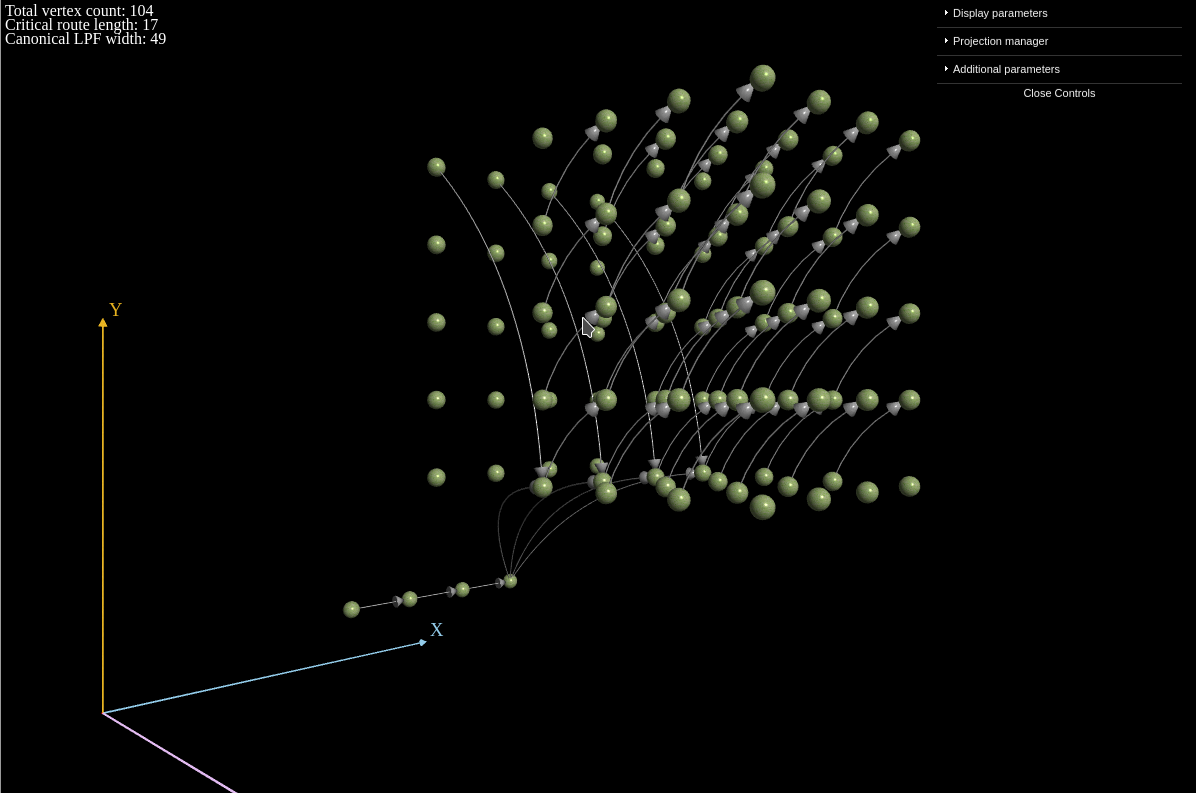
\includegraphics[scale=0.5]{src/graph_3d.png}\\
		Рис.1. Вид информационного графа в пространстве.
	\end{center}
	
	\begin{center}
		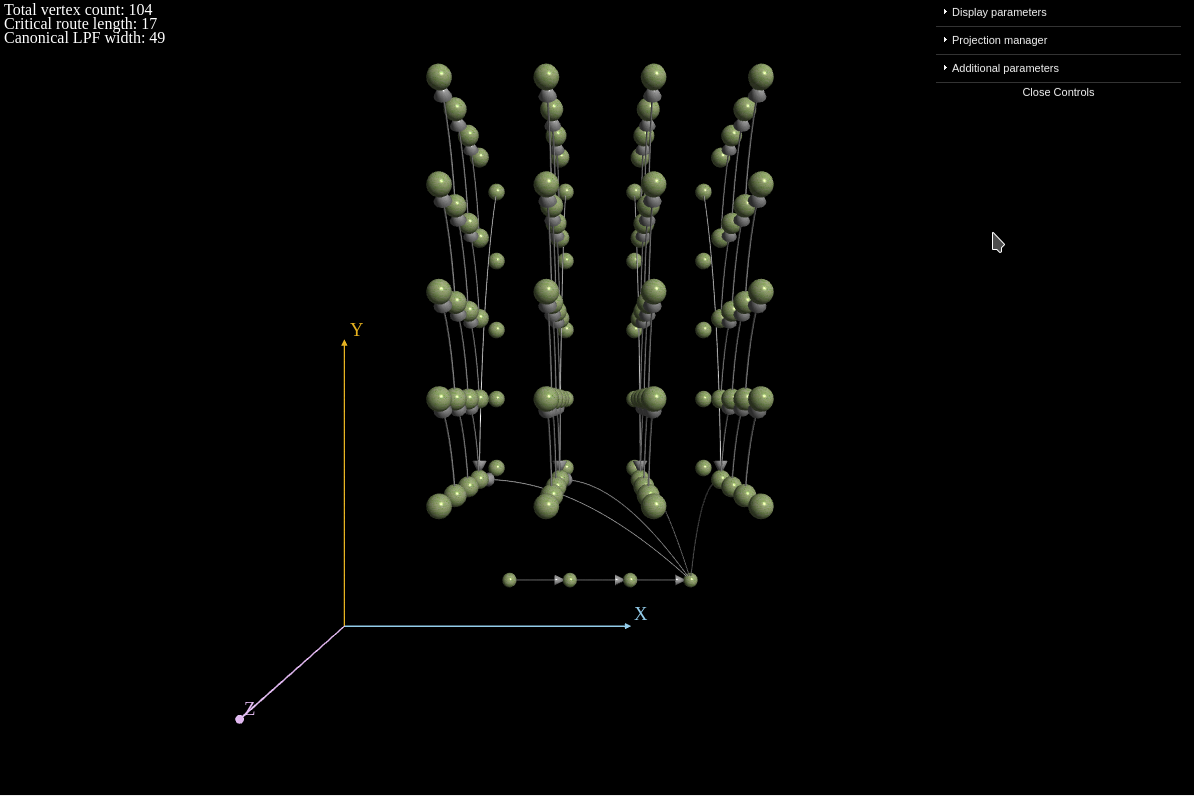
\includegraphics[scale=0.5]{src/graph_xy.png}\\
		Рис.2. Проекция информационного графа на плоскость XOY.
	\end{center}
	
	\begin{center}
		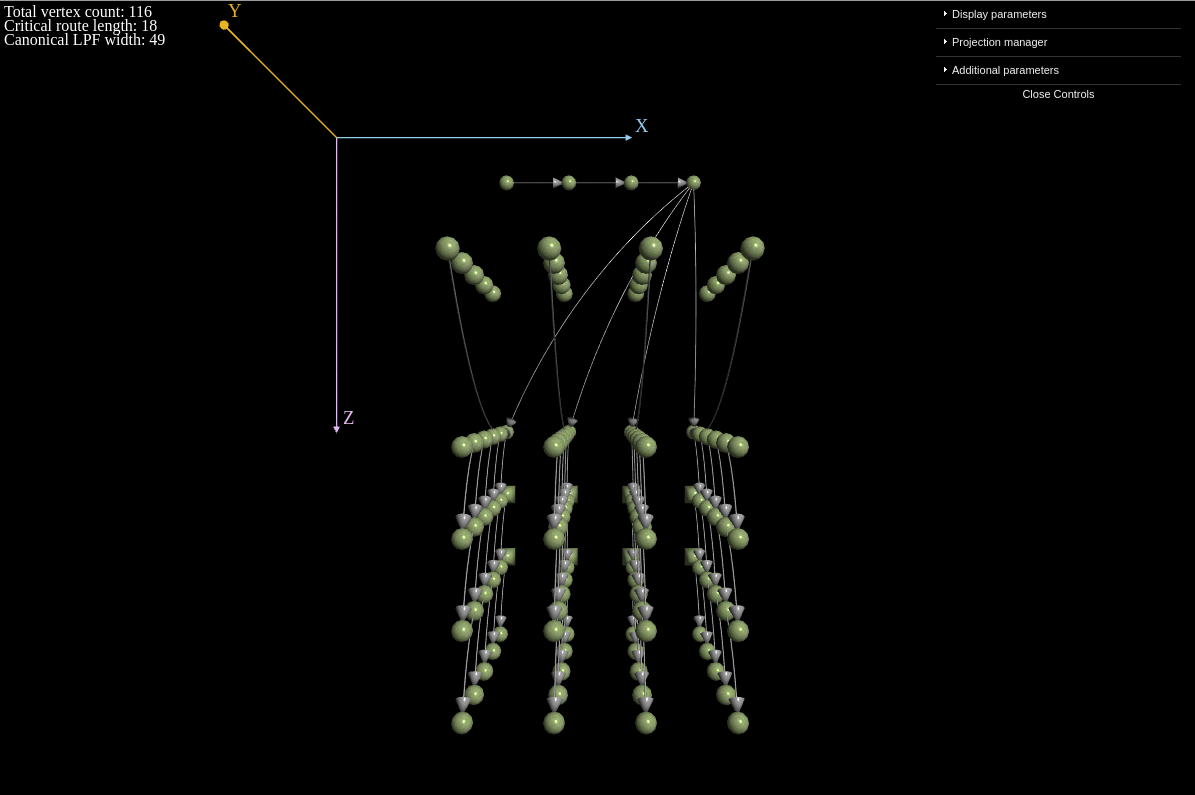
\includegraphics[scale=0.5]{src/graph_xz.png}\\
		Рис.3. Проекция информационного графа на плоскость XOZ.
	\end{center}
	
	\begin{center}
		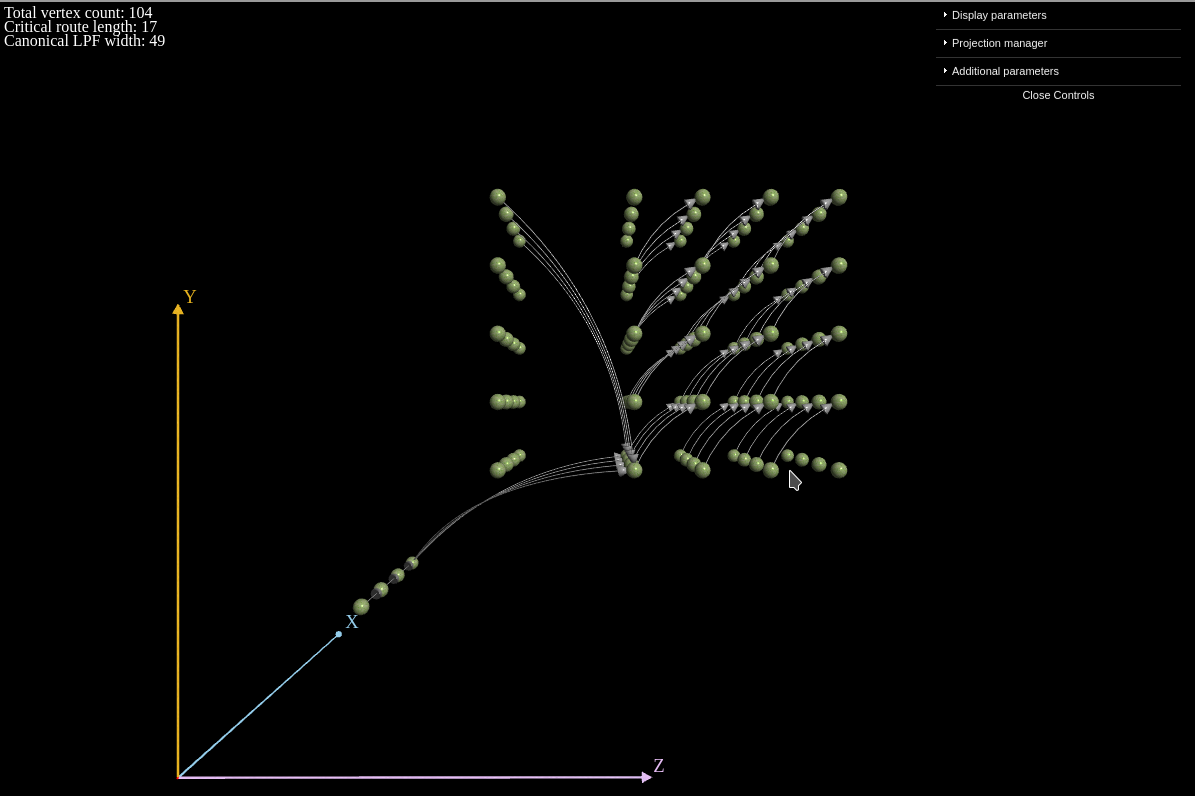
\includegraphics[scale=0.5]{src/graph_yz.png}\\
		Рис.4. Проекция информационного графа на плоскость YOZ.
	\end{center}

\section{Исследование свойств}

	\begin{itemize}
		\item Число вершин в информационном графе фрагмента программы при фиксированных значениях $N = 4$, $M = 5$: $104$. В общем случае формула имеет вид: $C = N + N \cdot M + N^2 \cdot M$.
		\item Длина (число дуг) критического пути в информационном графе при фиксированных значениях $N = 4$, $M = 5$: $7$. В общем случае формула имеет вид: $G = N + min\left(N - 1, M - 1\right)$.
		\item Ширина (максимальное число вершин на ярусе) ярусно-параллельной формы при фиксированных значениях $N = 4$, $M = 5$: $4$. В общем случае ширина $1 + NM + (N -1)N + (M - 1)N$, т.к. при построении ярусно-параллельной формы наибольшая ширина достигается на $1$-ом ярусе. Под шириной яруса понимается число вершин, из которых на данном ярусе не выходят ребра.
		\item Максимальная глубина вложенности циклов: $3$.
		\item Число различных типов дуг (тип дуг определяется направляющим вектором и длиной при фиксированных значениях параметров). При фиксированных значениях $N = 4$, $M = 5$ число различных дуг равно $4$. В общем случае количество различных дуг равно $3 + N$, т.к. в последнем цикле присутствует зависимость $A[i][1][1] от C[n + 1]: A[i][1][1] = B[i][m + 1] + C[n + 1]$.
		\item Наличие длинных дуг. Длинные дуги есть. Это дуги, образующие зависимость $A[i][1][1]$ от $B[i][m + 1]$ в последнем цикле. Дуги $A[i][1][1] - C[n + 1]$ не являются длинными, т.к. увеличение $M$ не влияет на эту зависимость, а при увеличении $N$ происходит добавление новых дуг, а не увеличение тех, которые были при $N - 1$. Таким образом, длинных дуг $N$ штук.
		\item Разметка параллельных циклов: предлагается полностью распараллелить второй блок циклов (оба цикла) и внешний цикл последнего блока циклов, т.к. нет обратной зависимости по $i$.
		
			\lstset{language=C}
			\begin{lstlisting}
	for(i = 2; i <= n+1; ++i)
	  C[i] = C[i - 1] + D[i];
	#pragma omp parallel for
	for(i = 2; i <= n+1; ++i)
	  #pragma omp parallel for
	  for(j = 2; j <= m+1; ++j)
	    B[i][j] = B[i][j];
	#pragma omp parallel for
	for(i = 2; i <= n+1; ++i){
	  A[i][1][1] = B[i][m + 1] + C[n + 1];
	  for(j = 2; j <= m+1; ++j)
	    for(k = 1; k <= n; ++k)
	      A[i][j][k] = A[i][j - 1][k - 1] + A[i][j][k];
			\end{lstlisting}
	\end{itemize}

	\newpage
	
	\section*{Список литературы}
	
	\begin{enumerate}
		\item В.В. Воеводин, Вл.В. Воеводин Параллельные вычисления // Спб:"БХВПетербург 2002
	\end{enumerate}

\end{document}